%%
% This file is modified based on the LAYOUT_E.TEX provided in REFMAN package. You can find the original REFMAN package at https://ctan.org/pkg/refman. This document only uses the LAYOUT_E.TEX as a template.

%%
% LAYOUT_E.TEX - Short description of REFMAN.CLS
%                                       99-03-20
%
%  Updated for REFMAN.CLS (LaTeX2e)
%
\documentclass[twoside,a4paper]{refart}
\usepackage{makeidx}
\usepackage{ifthen}
% ifthen wird vom Bild von N.Beebe gebraucht!
\usepackage{url}
\usepackage{graphicx}
\usepackage{xcolor}
\usepackage{listings}
\usepackage{csquotes}
\lstset{basicstyle=\ttfamily,
  showstringspaces=false,
  commentstyle=\color{red},
  keywordstyle=\color{blue}
}

\title{Misconduct Detection Project(MDP) Tool\\
Testing and Debugging Report No.1}
\author{Yucheng Xie \\
\today \\
Supervisor: Dr. Kyriakos Kalorkoti\\
Master of Science\\
School of Informatics\\
University of Edinburgh\\
Software Version: 1.0}

\date{}
\emergencystretch1em  %

\pagestyle{myfootings}
\markboth{Testing and Debugging Report No.1}%
         {Testing and Debugging Report No.1}
\makeindex 
\setcounter{tocdepth}{2}

%% Defines the bug name and bug ID here
% =====================================================
\newcommand{\bugfirst}{DET-001: Probability Calculation Error}
\newcommand{\bugsecond}{DET-002: JPlag Results Interpreting Error}


\begin{document}

\maketitle

\tableofcontents

\newpage


%%%%%%%%%%%%%%%%%%%%%%%%%%%%%%%%%%%%%%%%%%%%%%%%%%%%%%%%%%%%%%%%%%%%

\section{Summary} \label{sec:intr}
This \enquote{testing and debugging report} is used as a record for later developers referring. Each bug in this report has been illustrated by following three aspects:
\begin{enumerate}
\item The details of the bug. This part is mainly giving the details of the bug, including how to reproduce the bug.
\item The analysis of the bug. This part is mainly focusing on analyzing the bug and providing fixing solutions to the bug.
\item The test cases of the bug. This part is providing the test cases for verifying the bug is resolved.
\end{enumerate}

Especially, in the above information, later developers should always rerun the test cases of a bug if any code related to the bug is changed. Rerunning test cases could guarantee that later changes on the code are not making these bugs recur.

$\ $

Involved bugs in this report:
\begin{enumerate}
\item \bugfirst
\item \bugsecond
\end{enumerate}

\section{\bugfirst} \label{sec:step}
\subsection{Bug Report Part}

\subsection*{General Information}
\begin{table}[!h]
\begin{tabular}{|l|c|}
\hline
\textbf{Title} & Probability Calculation Error \\ \hline
\textbf{ID} & (detection package) DET-001 \\ \hline
\textbf{Priority} & Critical \\ \hline
\end{tabular}
\end{table}

\subsection*{Description}
When duplicating two identical files in the source folder, some ridiculous probability results such as 2 can be obtained.

\subsection*{How to Reproduce}
\begin{enumerate}
\item Set up the source folder with only 1 submission.
\item Duplicate the submission in the source folder. Now, we should have two identical submissions in the source folder.
\item Select one segment in the source file. Here we select the first function in the source file. However, selection of segments should not affect reproducing this bug.
\item Perform detection by clicking \enquote{Next} button on the \enquote{Selection} page.
\end{enumerate}

\subsection*{Screenshots}
\begin{figure}[!h]
\centering
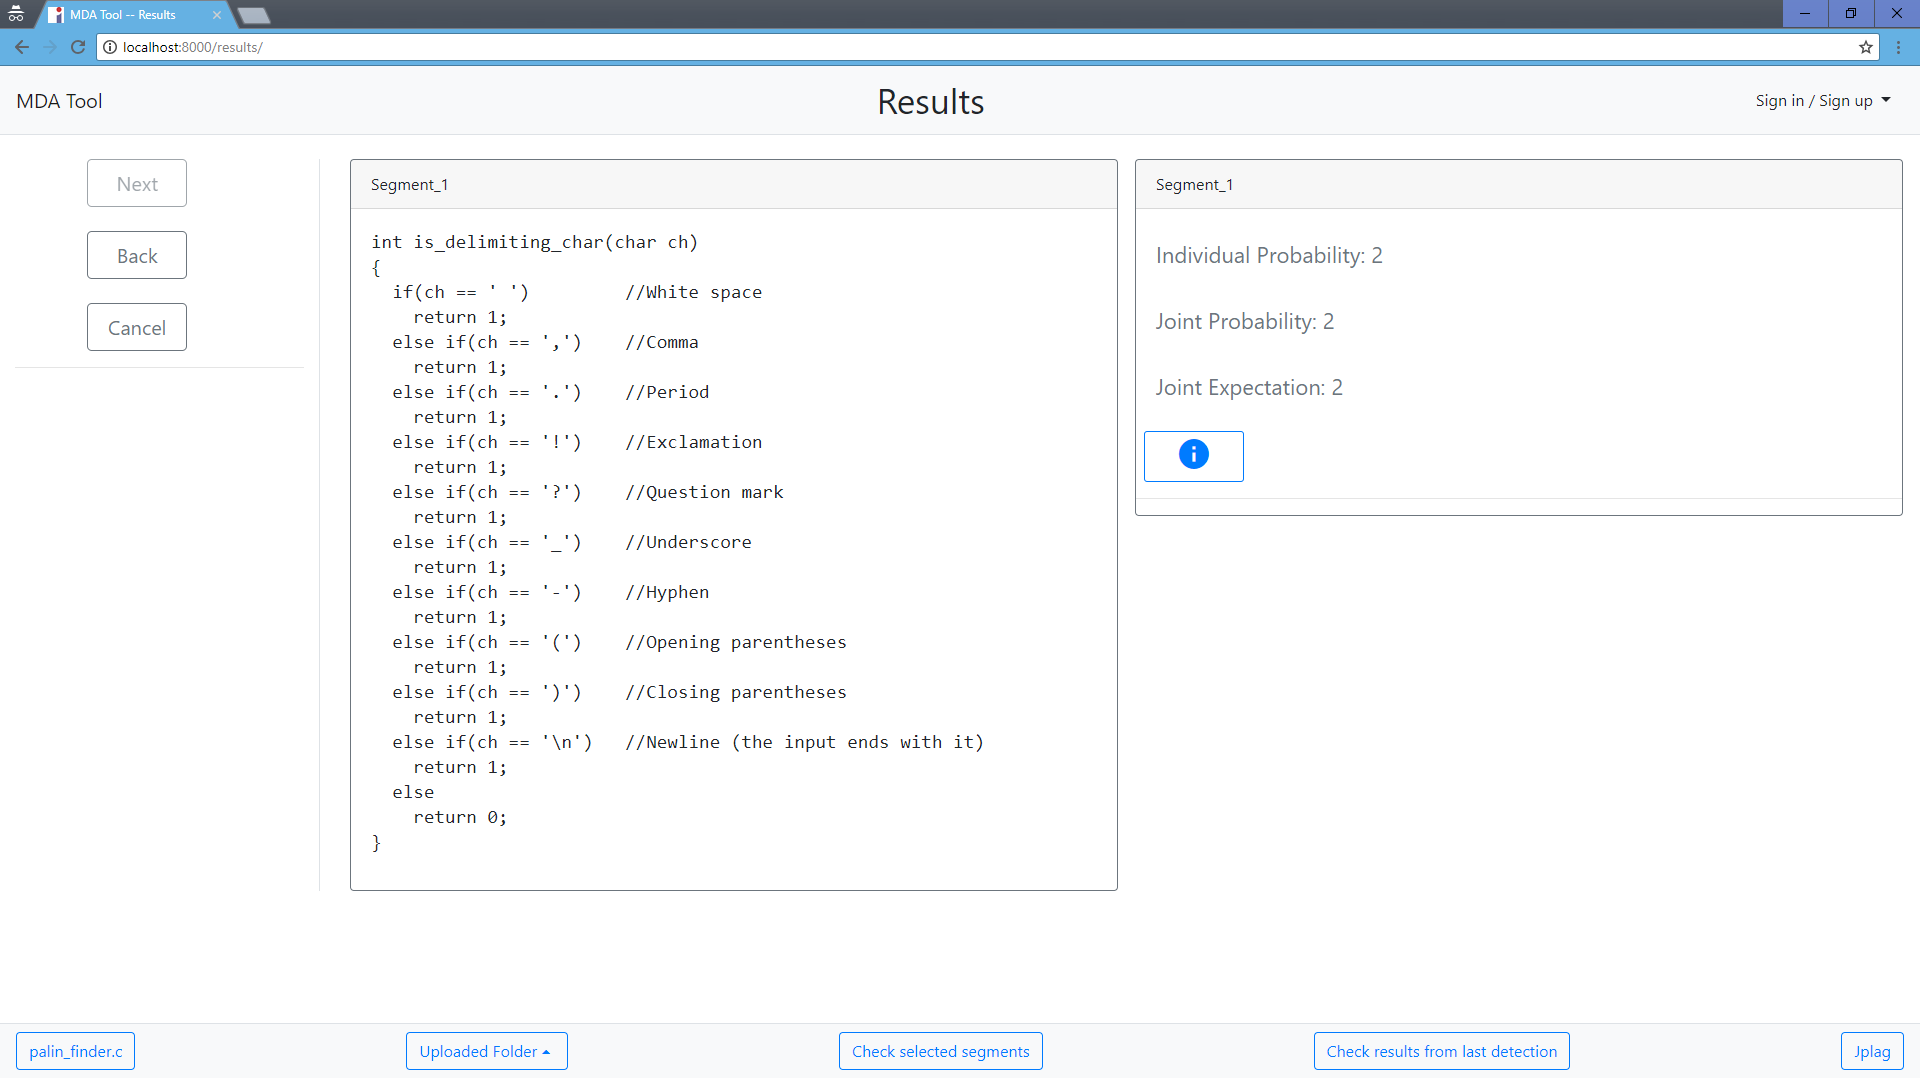
\includegraphics[width=12cm]{img/bug1.png}
\caption{\bugfirst $\ $ screenshot}
\label{fig:bug1_1}
\end{figure}

$\ $

\subsection{Bug Analysis Part}
As a result, we made a calculation error here in the code. We did not exclude the source file itself from the folder, which causes counts to be \enquote{2} in this case. We then exclude the source file from the source folder.

\subsection{Test Cases Part}
Test Case 1:

\begin{enumerate}
\item Set up a source folder, which contains exactly one submission.
\item Duplicate this submission, make sure the source folder contains two identical submission.
\item Select several segments randomly and perform detection.
\end{enumerate}
Expected Results for this Test Case: 

The results probabilities (both individual and joint) of all segments should always be \enquote{1}.

%% Bug 2
%=====================================================
\section{\bugsecond} \label{sec:step}
\subsection{Bug Report Part}

\subsection*{General Information}
\begin{table}[!h]
\begin{tabular}{|l|c|}
\hline
\textbf{Title} & JPlag Results Interpreting Error \\ \hline
\textbf{ID} & DET-002 \\ \hline
\textbf{Priority} & Critical \\ \hline
\end{tabular}
\end{table}

\subsection*{Description}
The result probabilities in some cases might become \enquote{0}. This bug is cased by an error in interpreting results obtained from JPlag.

\subsection*{How to Reproduce}
\begin{enumerate}
\item Set up the source folder with only 1 submission.
\item Duplicate the submission in the source folder. Now, we should have two identical submissions in the source folder.
\item Select \emph{More Than} one segments in the source file. Here we select the first two functions in the source file. However, which functions are selected should not affect reproducing this bug.
\item Perform detection by clicking \enquote{Next} button on the \enquote{Selection} page.
\end{enumerate}

\subsection*{Screenshots}
\begin{figure}[!h]
\centering
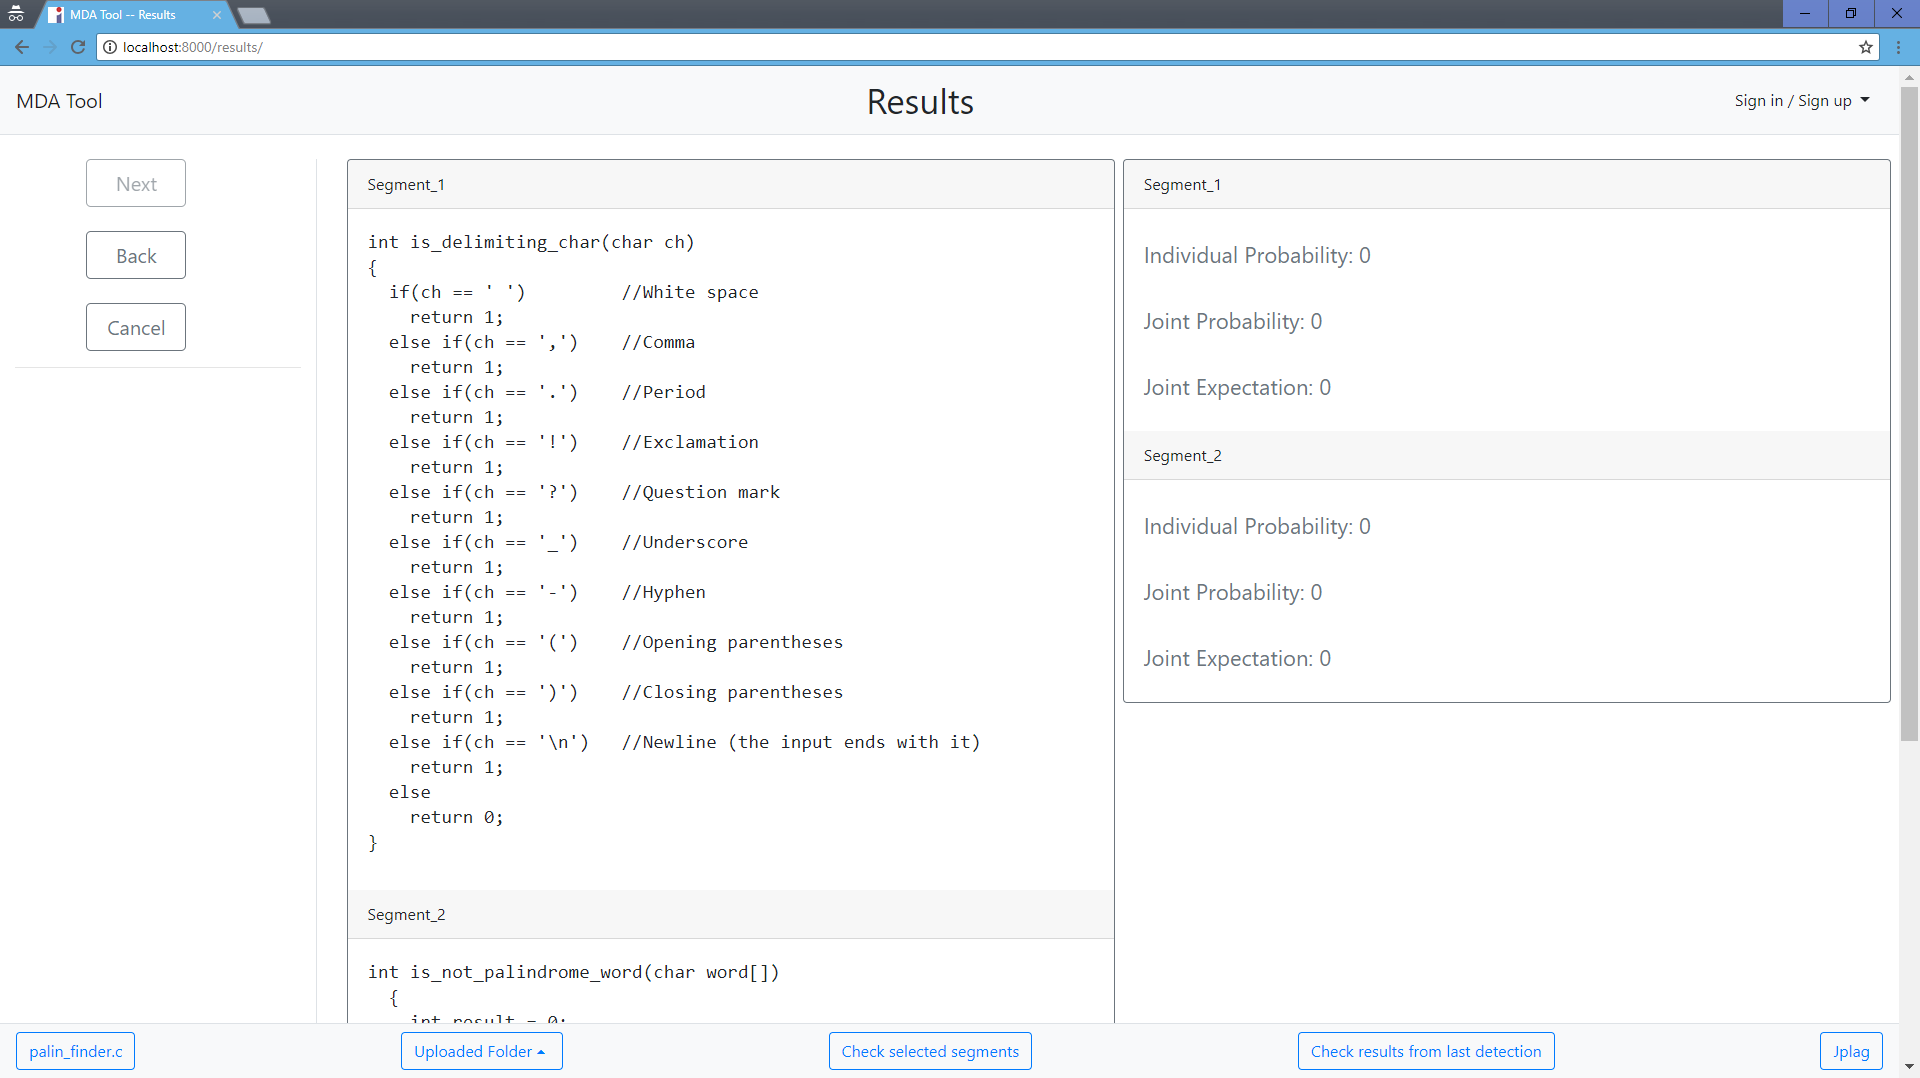
\includegraphics[width=12cm]{img/bug2.png}
\caption{\bugsecond $\ $ screenshot}
\label{fig:bug2_1}
\end{figure}

\subsection{Bug Analysis Part}
\begin{figure}[!h]
\centering
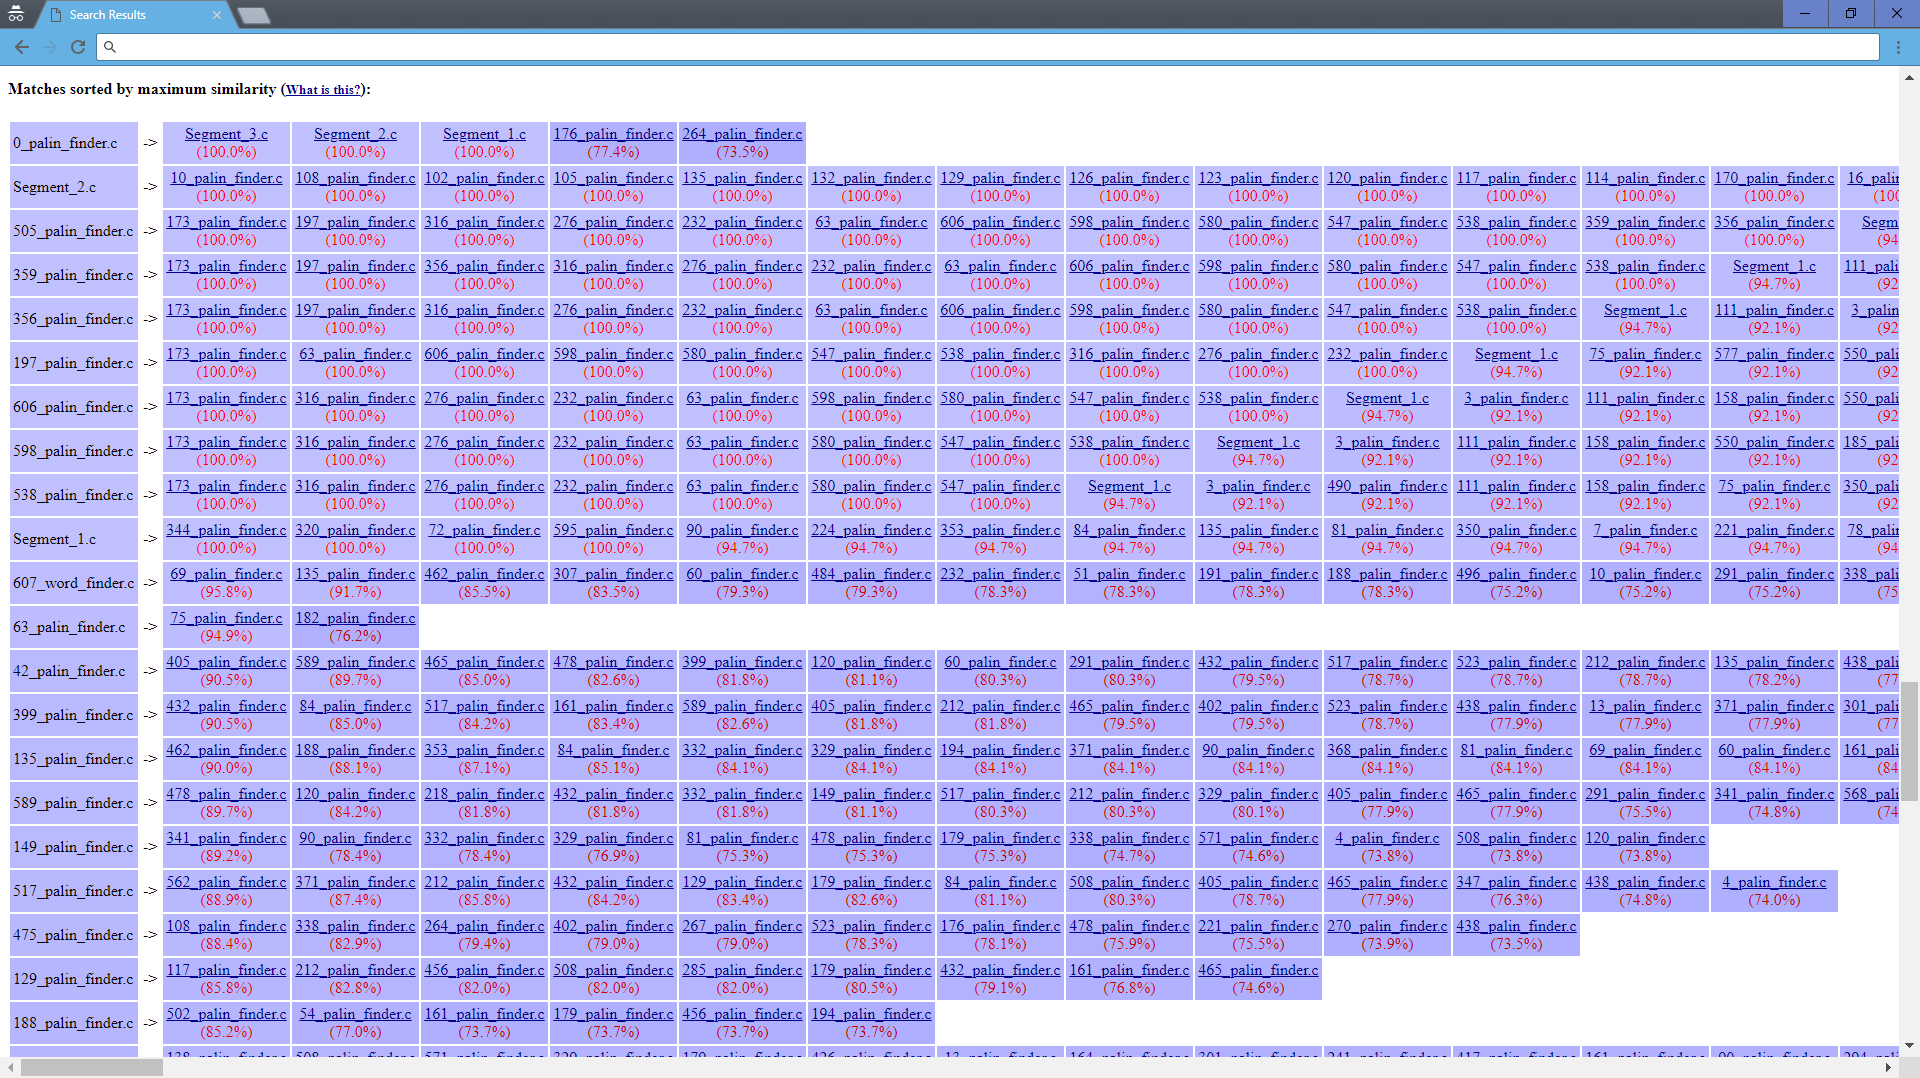
\includegraphics[width=12cm]{img/JPlag_1.png}
\caption{JPlag result index page screenshot}
\label{fig:bug2_ana_1}
\end{figure}

\begin{figure}[!h]
\centering
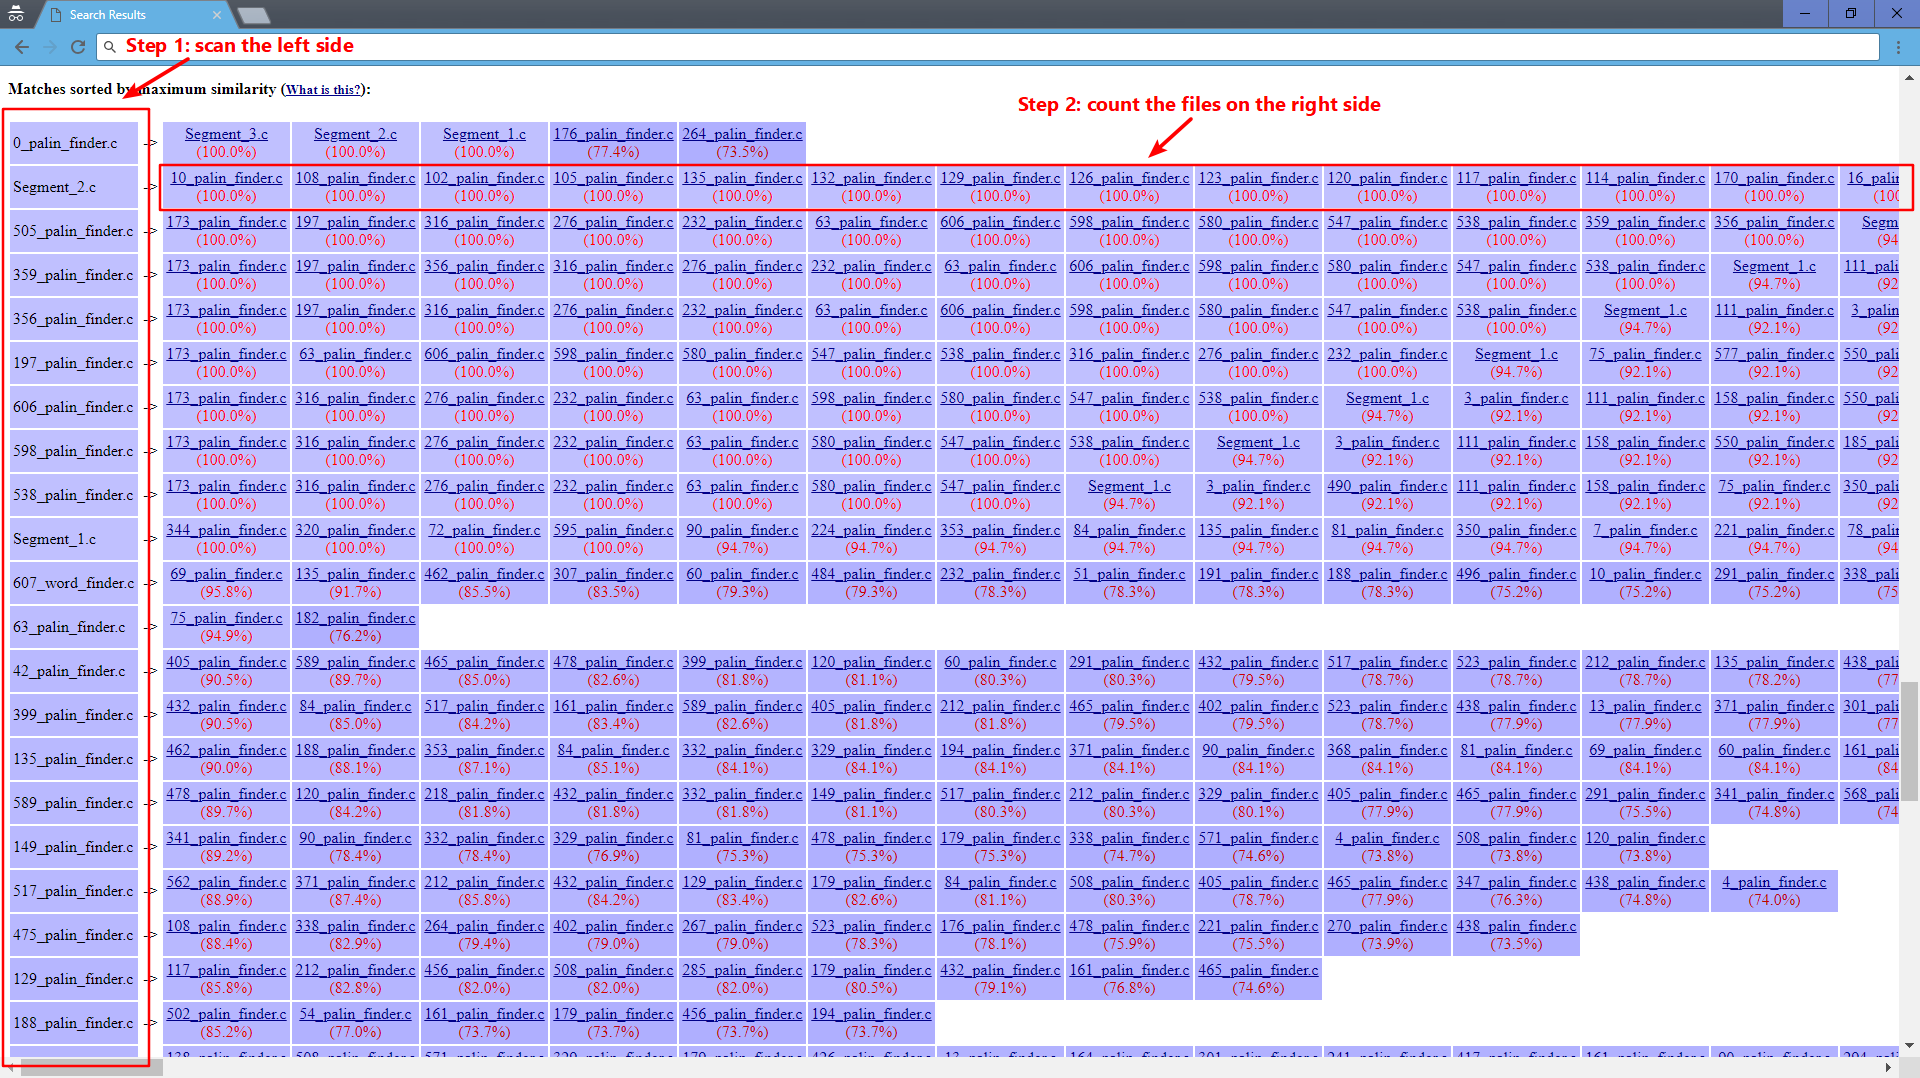
\includegraphics[width=12cm]{img/JPlag_2.png}
\caption{JPlag result index page screenshot with marks}
\label{fig:bug2_ana_2}
\end{figure}

\begin{figure}[!h]
\centering
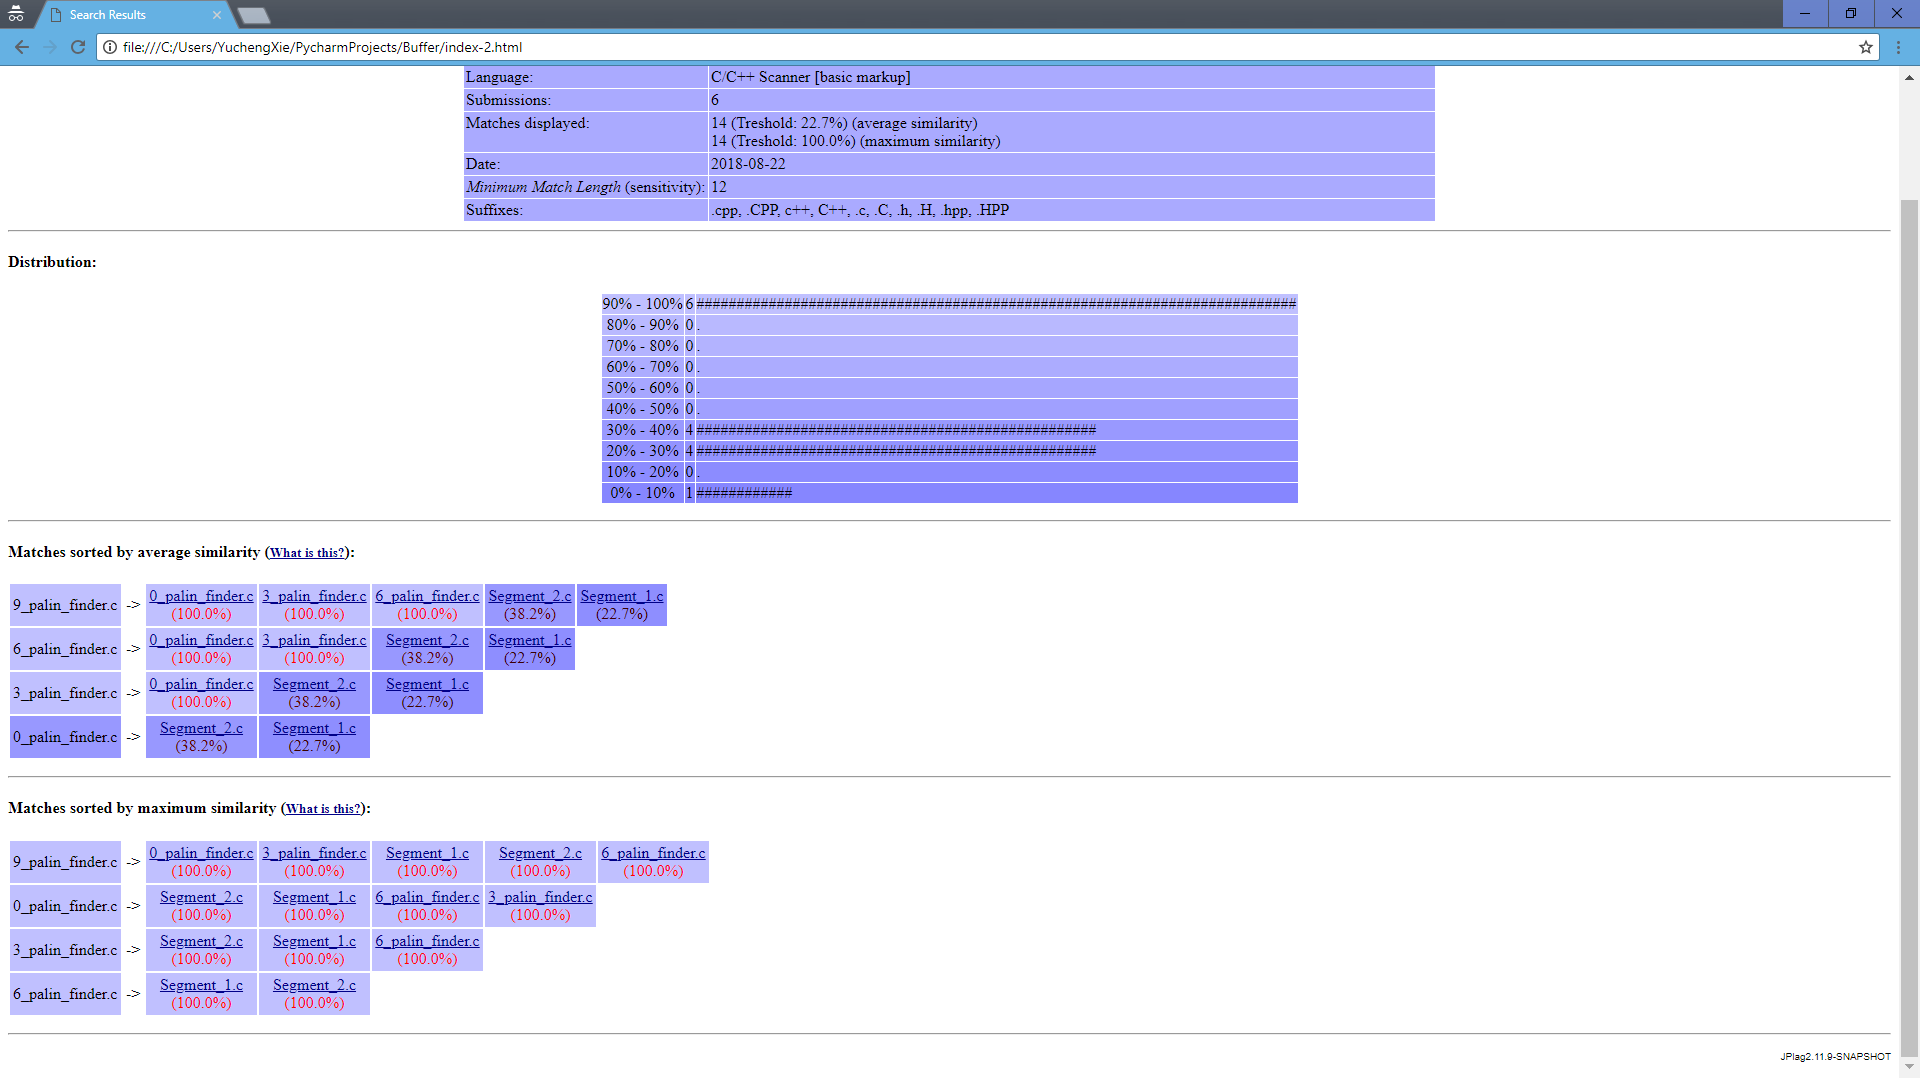
\includegraphics[width=12cm]{img/JPlag_3.png}
\caption{JPlag result index page which cases error screenshot}
\label{fig:bug2_ana_3}
\end{figure}

To illustrate how this bug is occurred, we need to mention how we extract information based on JPlag's results. We followed the following steps to obtain information from JPlag's results:

For example, the JPlag result index page usually looks like as shown in Figure \ref{fig:bug2_ana_1}. On this page, we scan left side first. Then, if we find any \enquote{Segment} on the left side, we just count the similar files on the right side. After that, we use this count number to calculate probabilities. (as shown in Figure \ref{fig:bug2_ana_2})

However, this is assuming that the \enquote{segments} will appear on the left side. If the \enquote{segments} are less suspect than other files, it actually will not appear on the left side. Like the situation we illustrated above. Under this situation, the JPlag final result index page will look like Figure \ref{fig:bug2_ana_3}. In Figure \ref{fig:bug2_ana_3}, we notice that all \enquote{segments} are not appearing on the left side. This is the reason why the \enquote{0} probabilities occur.

To resolve this bug, we need to consider the \enquote{segments} even if they only appear on the right side. We noticed that the JPlag will show every pairwise record for exactly one time. For example, assume that we have \enquote{file 1} and \enquote{file 2} are similar. If both of them are suspect enough to be shown on the left side, the record will appear exactly one time overall. That is, if this record appears at the right side of \enquote{file 1}, it then will not appear at the right side of \enquote{file 2} and vice versa.

Therefore, here to fix this bug, our solution should be counting both situation for one file. That is, if our segment appears on the left side, append what appear on the right side to the overall record of this segment. Then, if this segment appears on the right side for other files, append this record to the overall record of this segment.

\subsection{Test Cases Part}
Test Case 1:

\begin{enumerate}
\item Set up the source folder with exactly 1 submission. 
\item Duplicate the submission in the source folder for more than one time. Here we choose to duplicate for 3 times. Now, we should have four identical submissions in the source folder.
\item Select \emph{More Than} one segments in the source file randomly.
\item Perform detection by clicking \enquote{Next} button on the \enquote{Selection} page.
\end{enumerate}
Expected Results for this Test Case: 

The results probabilities (both individual and joint) of all segments should always be \enquote{1}. The joint expectation should be \enquote{3}.

\clearpage

\section*{Appendix}
\addcontentsline{toc}{section}{Appendix}

\appendix

\section{Explanation of Bug Priorities}
In this report, we divided all bugs into three different priority levels. They are:

\begin{enumerate}
\item Critical:

Something could case the whole system to be stopped or case the system producing wrong results.

\item Normal:

Something might affect later developing. Or something might case some further problems if it is not properly resolved.

\item Minor:

Annoying but not harmful to the functionalities. Such as layout displaying error in different browsers.
\end{enumerate}

\printindex

\end{document}
